\section{Hardware}

\subsection{Stepper motor}
En stepper motor, også ofte kaldt en “stepper” er en type af elektrisk motor som kan bruges til mange forskellige ting. En af fordelene ved at bruge en stepper motor i stedet for en DC motor er, at bevægelsen med stepper motor kan gøres meget præcist i forhold til en DC motor. Dette kommer sig af navnet “stepper motor”, da motoren ikke har en “flydende” kontinuerlig bevægelse, men bevæger sig frem i trin.\\

Bevægelsen bestemmes af magnetiske poler som tændes og slukkes alt efter hvilken retning og mængde af trin der ønskes, en stepper kræver altså en eller anden form for driver, dette kan som eksempel forekomme i form af en H-bro. Trin styres af to forskudte magnetiserede tandhjul som stemmer overens med en af de to sæt magnetiske poler, disse sidder forskudt på en sådan måde at når den ene aktiveres, trækkes det nærmeste sæt tænder med modsat polaritet frem, herefter tændes den anden pol for at rykke det andet sæt tænder frem\footnote{Video og artikel om stepmotorer: \url{https://youtu.be/0qwrnUeSpYQ} og \url{https://www.instructables.com/id/How-to-use-a-Stepper-Motor/} 
}. \\

I vores kredsløb har vi brugt stepmotorer til at kontrollere retningen på vores kanontårn, en som rotere tårnet om dens centrum, og en som styre vinklen på selve geværet. 

\subsection{DC motor}
En DC motor er simpel en elektromagnetisk motor som fungerer på det samme princip som en stepmotor. Ved at kontrollere mængden og “retningen” af strømmen som løber igennem denne motor kan motoren kontrolleres til et vist punkt. I modsætning til en stepmotor er det begrænset hvor præcist en DC motor kan styres, dog har den en flydende bevægelse samt er den mere enkel i sin funktion og er derfor lettere at kontrollere.\\

I stærk kontrast til en stepmotor har en DC motor kun to mulige forbindelsespunkter. Retning er baseret på hvordan strømforsyningen er koblet til, og hastighed er baseret på den spænding som der bliver tilført. Ved kun at have to forbindelsespunkter, samt at magneterne altid er tændt på samme tid bliver motoren langt mere enkel at bruge i forhold til en stepmotor da der ikke opstår problemer med paritet mellem de forskellige magnet elementer.



\subsection{H-bro}
En H-bro bliver brugt til at ændre strømmens retning gennem et kredsløb. Ved at styre strømmen gennem fire porte kan man tænde og slukke for ønskede elementer baseret på outputs fra en arduino. I dette projekt bruger vi H-broen til at tænde for de individuelle magneter på vores stepmotorer for at skabe, og styre, rotation. At bruge en H-bro skaber også en mængde problemer, foruden problemer med opsætning og software, falder den spænding som bliver sendt til motoren med omkring 2 volt ved brug af en standard arduino H-bro (L298N\footnote{Data om standard Arduino H-bro, Underemnet: L298N \url{https://howtomechatronics.com/tutorials/arduino/arduino-dc-motor-control-tutorial-l298n-pwm-h-bridge/}}). 

Dette kan resulterer i at motoren er knap så stærk, da dennes styrke afhænger af hvor meget strøm elektromagneterne får. 


\subsection{Knapper}
I dette projekt er der blevet brugt flere knapper. Knapper kan bruges til at registrere et brugerinput. Knapper bliver ofte brugt når man skal bruge et simpelt input. F.eks. bruges knapper i dette projekt til at registrere, hvornår hardball pistolen skal skyde ud fra brugerens tryk.\\

Knapper fungerer ved at en mikrocontroller kan afmåle en spændingsforskel som knappen skaber. En ATMega328p kan afmåle disse spændingsforskelle gennem de digitale input / output. 

\subsection{Relæ}
Et relæ er en kontakt, som kan videresende strøm, hvis det aktiveres. Det bliver aktiveret ved at strømmen skaber et elektromagnetisk felt, som er stærkt nok til at lukke kontakten inde i relæet.\\

Vi bruger relæet til at tænde og slukke for skydemekanismen i airsoft-geværet ved hjælp af strømmen fra mikrocontrolleren, som tænder for relæet, der derefter lader strømmen fra geværets batteripakke gå igennem, hvilket resulterer i affyring.



\subsection{BlueSMiRF}
I dette projekt bruger vi flere bluetooth kommunikationselementer af typen “BlueSMiRF Silver”. Disse er simple, kommandobaserede kommunikationsmodemmer, som kan bruges gennem arduino. Dette gør det muligt at bruge dem i kombination med mange af de andre komponenter i vores produkt.\\

Bluetooth-kommunikation fungerer ved svage, sekvensbaserede radiosignaler mellem forskellige enheder. Dette kommer sig af, at det originalt var tiltænkt som en trådløs løsning til overførsel af data fra enheder som mobiltelefoner, som ikke har adgang til en høj spænding. Enheder inddeles i de to kategorier “slave” og “master”. Masteren er den enhed som starter kommunikationen mellem de forbundne enheder. Den bestemmer også, hvornår slaverne må sende deres signal for at holde selve kommunikationen synkron mellem slaverne og masteren\footnote{Information om Bluetooth: \url{https://www.elprocus.com/how-does-bluetooth-work/} 
}.\\

I vores projekt har vi en master forbundet til vores controller og en slave forbundet til selve tårnet, her sender masteren så de input den får gennem seriel kommunikation til slaven som er forbundet på selve tårnet. Slaven modtager et enkelt tegn baseret på et knaptryk, som den så udføre en handling ud fra, dette kunne for eksempel være at fortælle stepmotoren at den skal køre en enkelt omgang.\\


\subsection{Accelerometer}
Et accelerometer er en elektronisk komponent som kan måle sin egen tyngdeacceleration. Mange accelerometerer kan aflæse sin tyngdeacceleration på tre akser (x, y og z). \\[0.5cm]

Man kan bruge et accelerometer til at bestemme et legemes rotation i rummet.\\[0.5cm] 

I dette projekt har vi brugt et accelerometer til at bestemme hældningen på vores gevær, og den har haft til opgave at stoppe geværet fra at hæve eller sænke sig for meget ved kombineret brug af accelerometer og interrupt i kode. Ved at vurdere sin placering har accelerometeret kunne bestemme om geværet er oversteget nogle forudbestemte maksimums- og minimumsværdier for geværet hældning, og har så, baseret på disse værdier, stoppet geværet i at hæve eller sænke sig mere end hvad er tilladt.



\subsection{Spændingsregulator}
En spændingsregulator virker som en zenerdiode, der kun tillader strøm op til en bestemt spænding at løbe igennem. Zenerdioder adskiller sig fra normale dioder ved, at de ikke prøver at spærre for alt strøm, men i stedet kun spærrer for strøm, som overstiger spændingsgrænsen.\\

Vi har i projektet brugt spændingsregulatoren LM7805, da denne korrekt nedskalerer vores strømkilde (9V) til de 5V en ATMega328p må få. Mere om kredsløbet, som komponenten indgår i kan findes under afsnittet om mikrocontrollerens el-diagram.



\subsection{Mikrocontroller (ATMega328p)}

ATMega’en er en programmerbar mikrocontroller, der er standardchippen i en Arduino UNO, hvilket betyder at den kan programmeres igennem Arduino IDE’en. Mikrocontrolleren har 28 pins, hvor af 13 er digitale pins (PD\# og PB\#) og 6 kan bruge PWM (pulse width modulation). Derudover har mikrocontrolleren 8 analoge pins (PC\#), hvor PC6 også er controllerens reset-pin, samt 2 VCC, 2 GND og en reference spænding (AREF).\\


\begin{figure}[H]
\centering
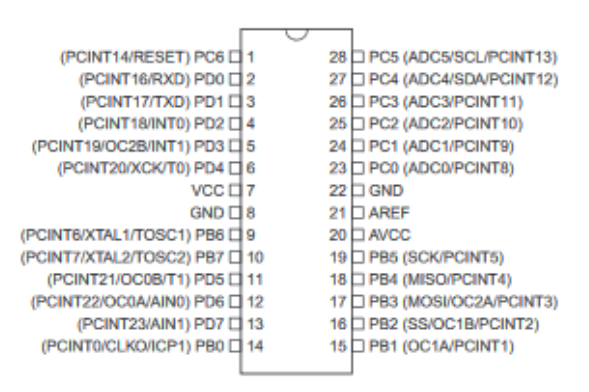
\includegraphics[scale=0.8]{Billeder/Mikrocontroller_pins.png}
\caption{Billede af ATMega328p's pin layout.}
\label{fig:ATMega_pin}
\end{figure}

Vi har i modsætning til tidligere projekter brugt en ATMega328p uden, at den sidder fast i en Arduino. Hvis denne sættes korrekt op, kan den dog udføre de samme opgaver, selvom dens programmering kompliceres ved, at den enten skal fastspændes i en Arduino hver gang, eller have en forbindelse mellem Arduino’ens TX og RX og ATMega’ens RX og TX (PD0 og PD1). Hvordan ATMega’en sættes op udenfor en Arduino kan ses under det næstkommende el-diagram afsnit.



\subsection{Krystaloscillator}
Vi bruger en 16 MHz krystaloscillator til at holde styr på ATMega’ens tidstagning. Krystallen virker ligesom en oscillator, da den bringes i stabile svingninger af strømmen fra mikrocontrolleren. Krystallens store stabilitet gør den i stand til at holde tiden ekstremt præcist, hvilket gør den ideel, hvis dele af ens kode kræver tidsstyring, som f.eks. præcise delays. \\

Mere om vores brug af krystaloscillatoren kan findes i afsnittet om mikrocontrollerprintet.

\subsection{El-diagrammer}
\subsubsection{Mikrocontrollerprint}

\begin{figure}[H]
\centering
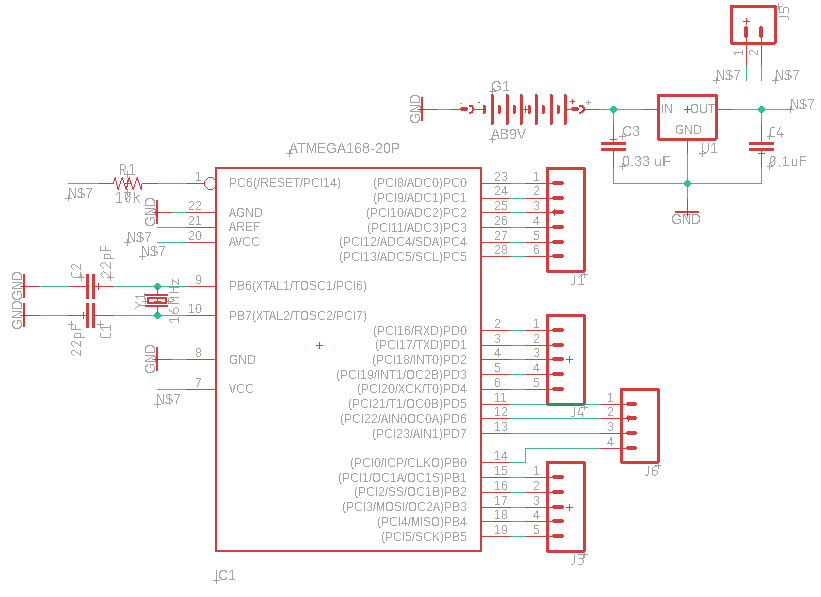
\includegraphics[scale=0.8, angle=90]{Billeder/El-diagram.PNG}
\caption{El-diagram over mikrocontrollerprint.}
\label{fig:El_diagram_mikro}
\end{figure}

Selve mikrocontrollerprintet består af 2 forbundne kredsløb. Det første er selve ATMEGA’en, som er udstyret med en krystaloscillator (Y1 på figur \ref{fig:El_diagram_mikro}), som er yderligere forklaret under hardware-afsnittet. Der er forbundet 2 kapacitorer mellem krystaloscillatoren og GND for at forbedre strømmens stabilitet. Krystaloscillatorens størrelse (16 MHz), samt kapacitorernes størrelse (22 pF) er baseret på ATMega’ens datablad, hvor disse er foreslået\footnote{ATMega datablad, afsnit 9.4: \url{http://ww1.microchip.com/downloads/en/DeviceDoc/ATmega48A-PA-88A-PA-168A-PA-328-P-DS-DS40002061A.pdf}}.\\

Derudover er der lavet huller til alle ATMega’ens resterende pins, så de kan bruges frit, ligesom på en Arduino. Ligesom det kan ses på el-diagrammet er ATMega’ens 2 GND pins forbundet til pladens GND og de to VCC pins, samt AREF er forbundet til den regulerede 5 volts kilde. Arduino’ens reset-pin er forbundet til 5 volts kilden igennem en 10 kΩ resistens, så spændingen forhindrer ATMEGA’en i at genstarte af sig selv.\\

Det andet, mindre kredsløb på mikrocontrollerprintet er spædningsregulatoren, som kan ses øverst til højre på figur \ref{fig:El_diagram_mikro}. Denne er tilstede, da mikrocontrolleren ikke må få mere end 5V. De to kapacitorer, som er tilsluttet selve spændingsregulatoren sørger for bedre stabilitet og er tilføjet, da dette var opfordret i komponentens datablad, hvis man vil have et konstant 5V output\footnote{M7805 datablad, side 7: \url{https://www.sparkfun.com/datasheets/Components/LM7805.pdf}}.

\subsection{PCB-layout}

\begin{figure}[H]
\centering
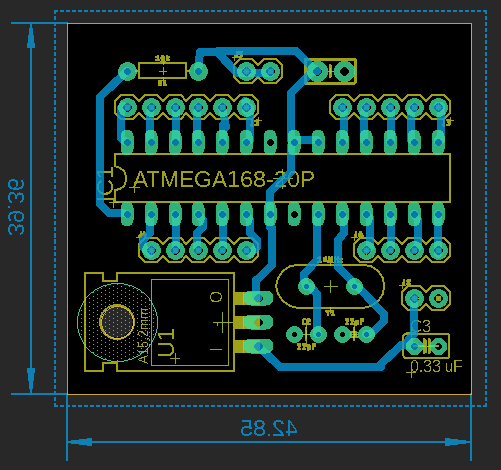
\includegraphics[scale=0.8]{Billeder/PCB_uden_kobber.PNG}
\caption{PCB-layout med angivede mål. Uden kobber på pladen.}
\label{fig:PCB}
\end{figure}

Layout’et er lavet i Eagle ud fra el-diagrammet på figur \ref{fig:PCB}. Alle komponenterne er placeret, så de fylder så lidt som muligt, men samtidig er mulige at lodde præcist i hånden. Som det kan ses på figur \ref{fig:PCB}, har vores mikrocontrollerprint dimensionerne: 42,85 x 39,36 mm.

\begin{figure}[H]
\centering
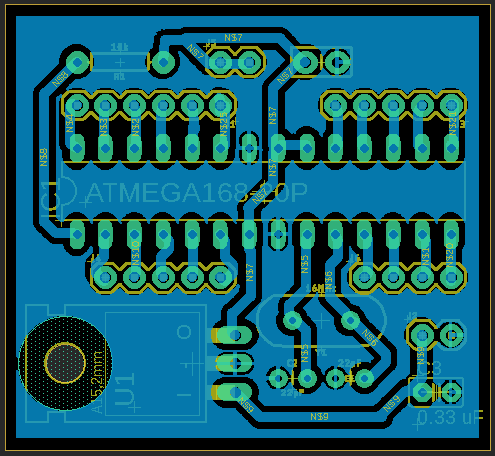
\includegraphics[scale=0.8]{Billeder/PCB_med_kobber.PNG}
\caption{PCB med kobber (GND) på pladen.}
\label{fig:PCB_kobber}
\end{figure}

Som illustreret på figur \ref{fig:PCB_kobber}, er der én samlet GND på pladen, som alt er forbundet til. Dette sparer meget plads, hvis sammenlignet med en løsning, hvor f.eks. en Arduino skulle have sin egen separate GND. Hvis man tænker på at hele mikrocontrollerprintet, egentlig bare er en simpel Arduino, giver det også mening at den skal være så lille som muligt, da dette er den “hjemmelavede” Arduinos største fordel, hvis sammenlignet med en standard Arduino UNO. En Arduino UNO vil f.eks. ikke kunne passe ind i en kompakt controller, mens dette mikrocontrollerprint ville kunne pakkes meget kompakt med dets minimale dimensioner.





